\documentclass{article}

\usepackage[a4paper, lmargin=10mm, rmargin=70mm]{geometry}
\usepackage{amsmath}
\usepackage{amsthm}
\usepackage{amssymb}
\usepackage{graphicx}

\title{ICS343 Subjective Part Summary}
\author{Alfaifi, Ammar}
\date{}

\begin{document}

\maketitle


\section{TCP/IP Protocol Suit}%
\label{sec:TCP}
\begin{itemize}

  \item Transmission Control Protocol/Internet Protocol (TCP/IP) is a protocol suit, meaning a set of functionalities
        provided between each layer.
  \item It is built in layer structure where the each layer takes services from the one bellow it,
        and provides services to the above it.
  \item Application, Transport, Network, Data link, Physical
        \begin{itemize}
          \item \textbf{Physical}: carries individual bits in a frame. communication between two devices
                in the this layer is still logical. under this layer is the transmission medium; carring
                electrical or optical signals. Logical unit is \textit{bit}
          \item \textbf{Data link}: Any protocol that takes datagram and carries it in the link is suffice
                for this layer. This layer takes datagram encapsulate it into a \textit{frame}. hop-to-hop communication.
          \item \textbf{Network}: is responsible for creating a connection between the source and destination computers. It's
                host-to-host communication and routing the packet to best path. It includes the main protocol, Internet Protocol (IP),
                which defines a packet called \textit{datagram}.
          \item IP is connectionless, that provides no flow control, no error control, and no congestion control services.
                It provides unicast  (one-to-one), and multicast (one-to-many) routing protocols.
                This layer has auxiliary protocols: ICMP helps IP to report some problems when routing a packet,
                DHCP helps IP to get the network-layer address's for a host, ARP help IP to find the data-link layer address
                of a host or a router given the network-layer address.
          \item \textbf{Transport}: the lgical connection is end-to-end. The packet is called a segment or user datagram.
                It has Transmission Control Protocol (TCP), which is a connection-oriented that established a logical connection
                before sending data. User Datagram Protocol (UDP), is a connectionless, which is simple and fast.
          \item \textbf{Application}: Logical connection is end-to-end. They exchange \textit{messages}.
                The communications is between two \textit{processes}. Examples: HTTP, SMTP, FTP, SSH, DNS is used by other
                protocols to find the network-layer address of a host.

          \item well-known ports : 0 - 1023, controlled by ICANN.
          \item registered ports: 1024 - 49151, not controlled by ICANN, but can be registered.
          \item dynamic ports: 49152 - 65535, as temporary or private ports.
        \end{itemize}

\end{itemize}

\section{Transport-Layer Protocol}%
\label{sec:TLP}

\subsection{Stop-and-Wait Protocol}%
\label{subsec:stop-and-wait protocols}

\begin{itemize}
  \item Both sender and receiver use sliding window of size 1.
  \item sends one packet at a time, and waits for an ACK.
  \item every sent packet, a timer starts.
  \item ACK value is the sequence \# of next packet.
  \item the sequence numbers are: 0, 1, 0, 1, $\dots$
\end{itemize}

\subsection{Go-Back-N Protocol (GBN)}%
\label{subsec:GBN}

\begin{itemize}
  \item it tries to send many packets while waiting for an acknowledgment.
  \item ACK \# is \textit{cumulative}; the sequence \# of next packet.
  \item window size up to $2^m -1$.
  \item $S_f$ first outstanding, $S_{n}$, $S_{size}$
  \item from $S_{f}$ to $S_{n}-1$: packets sent but not acknowledged.
  \item from $S_{n}$: packets to be sent
  \item window slides when an error-free ACK, $S_{f} \leq \text{ackNo} \leq S_{n}$, received.
  \item receive window is always of size 1.
  \item receive window, $R_{n}$, next packet expected.
  \item there is only one timer, for the first outstanding packet.
  \item at the timer expiration, \textit{all} outstanding packets are resent.
  \item window is full if $S_{n} = (S_{f} + S_{size}) \mod 2^{m}$
  \marginpar{
    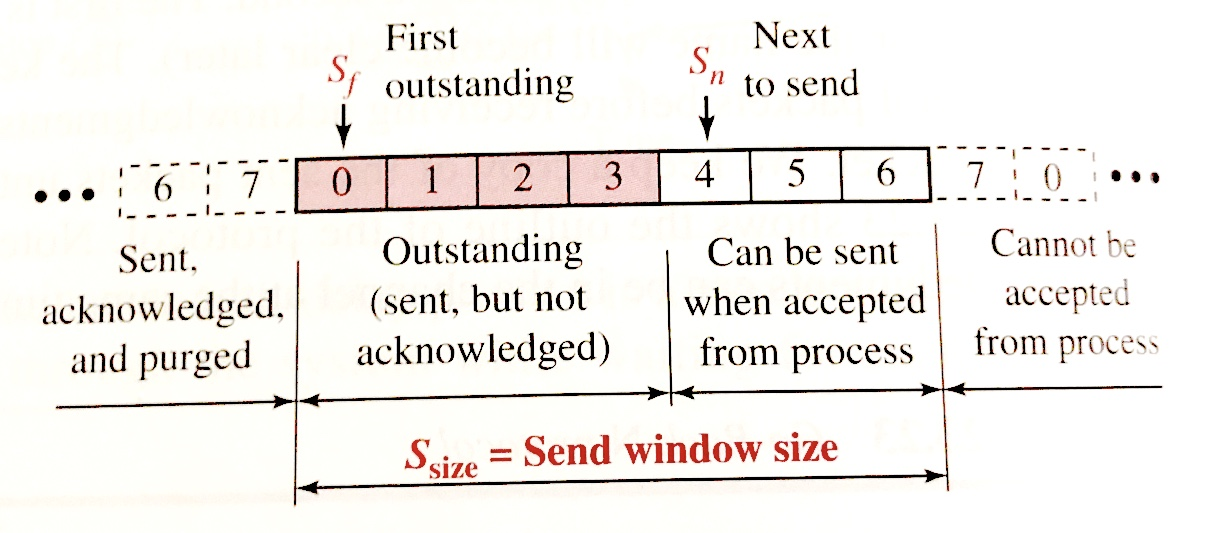
\includegraphics[width=0.5\textwidth]{figures/wind.jpeg}
        }
  \item in receiver side, with error-free ACK, $S_{f}=\text{ackNo}$. if $\text{ackNo}=S_{n}$ stop timer.
\end{itemize}

\subsection{Selective-Repeat Protocol}%
\label{subsec:SRP}
GBN is inefficient if network loses a lot of packets.
\begin{itemize}
  \item sender window size is $2^{m-1}$, the receive window should equal the send window
  \item In reliable protocols, receiver never deliver packets out of order to the application layer.
  \item ackNo is the sequence \# of the received packet; ackNo isn't cumulative.
        It does \textbf{not} mean all packets with sequence \# less than ackNo are received.
\end{itemize}

\subsection{Bidirectional Protocols: Piggybacking}%
\label{subsec:bidre}

The idea is that, we make the packets that carries data, to carry also the ackNo at
the same time. So that we don't overwhelm the network with packets carring just ackNo.



\section{HyperText Transfer Protocol}%
\label{sec:HTTP}

\begin{itemize}
  \item The server uses the port 80, and 443 for secured one (HTTPS).
  \item form v1.1 persistent mode is the default.
  \item In the nonpersistent connection: the client opens a TCP connection and sends a request.
        The server responds and closes the connection. The client reads and colses the connection.
  \item Methods in the header message:
        \begin{itemize}
          \item GET: requests a doc.
          \item HEAD: requests info about a doc.
          \item POST: sends info to the server.
          \item PUT: sends a doc to the server.
        \end{itemize}
  \item Some request headers:
        \begin{itemize}
          \item user-agent: the client program.
          \item accept: media formats client understands.
          \item host: host and port number of client.
          \item if-modified-since: last update of file; this tell the server
                to send the data only if it was modified since this data.
        \end{itemize}
  \item some response headers:
        \begin{itemize}
          \item server: info about the server.
          \item last-modified: the date of last change.
          \item content-type: media type.
        \end{itemize}
\end{itemize}

\section{Electronic Mail (Email)}%
\label{sec:Email}

\begin{itemize}
  \item US: user agent, MTA: message transfer agent, MAA: message access agent.
  \item US, using MTA client, sends a msg to the MTA server then to a spool (a queue)
        then to MTA client in the server then to the MTA server of reciever then to
        the receiver UA mail box them to MAA server then to MAA client.
  \item it needs 2 UAs, 2 pairs of MTAs (slient \& server), and a pair of MAAs.

\subsection{Message Transfer Agent: SMTP}%
        \label{subsec:SMTP}

        Some of Simple Mail Transfer Protocol (SMTP) commands:
        \begin{itemize}
          \item HELO: sender's host name
          \item MAIL FROM: sender of the msg
          \item RCPT TO: the recipient.
          \item DATA: message body.
          \item QUIT: ends the message
        \end{itemize}

\subsection{Message Access Agent}%
\label{subsec:MAA}
\begin{itemize}
  \item Post Office Protocol (POP) is very simple to get the mails form the server mail boxes.
  \item Internet Mail Access Protocol (IMAP) it can check the header of a msg, search, or partially
        download a msg.
\end{itemize}
  \item Multipurpose Internet Mail Extension (MIME) is to help sending non-textual data.
  \item Base64 is one of the methods to encode data into ASCII characters.
        Base64 means $\log_{2}64=6$ bits, converts each 6 bits into their ASCII chars.
  \item Note that 0 corresponds to \textbf{A}, so \textbf{a} is 26 and so on.
  \item the sequence: \textbf{A-Z}, \textbf{a-z}, \textbf{0-9}
\end{itemize}



\end{document}
